\documentclass{article}




\usepackage{amsmath}
\usepackage{amssymb}
\usepackage{amsthm}
\usepackage{listings}
\usepackage{color}
\usepackage{algorithmicx}
\usepackage{algpseudocode}

\newtheorem*{theorem}{Theorem}

\definecolor{dkgreen}{rgb}{0,0.6,0}
\definecolor{gray}{rgb}{0.5,0.5,0.5}
\definecolor{mauve}{rgb}{0.58,0,0.82}

\lstset{frame=tb,
  language=Java,
  aboveskip=3mm,
  belowskip=3mm,
  showstringspaces=false,
  columns=flexible,
  basicstyle={\small\ttfamily},
  numbers=left,
  numberstyle=\color{gray},
  keywordstyle=\color{blue},
  commentstyle=\color{dkgreen},
  stringstyle=\color{mauve},
  breaklines=true,
  breakatwhitespace=true,
  tabsize=3
}


\usepackage{Sweave}
\begin{document}
\setkeys{Gin}{width=1.0\textwidth}


\begin{titlepage}
\vspace{2cm}
\begin{center}
\textbf{Assignment 1}\\
\vspace{0.5cm}
Empirical Analysis of an Algorithm\\
\vspace{1.5cm}
\textbf{Oliver Caddie}\\
\vfill

CAB203\\
Queensland University of Technology\\
11/4/19
 
\end{center}
\end{titlepage}





\tableofcontents


\pagebreak


\section{Algorithm Description}
\subsection{Preliminary Overview}
The algorithm shown below searches the given array of numbers, $a$, for the "median" value: the value located at $\lceil \frac{n}{2} \rceil$ in the sorted array, $a'=(a,\leq)$ (Assuming $n > 0$). It achieves this by iterating through $a$ and counting how many elements are equal ($e$) and how many are less than ($s$) each element until it reaches one that satisfies the condition:
\begin{align*}
s < \Big\lceil \frac{n}{2} \Big\rceil \leq s + e
\end{align*}
The above inequality will be satisfied by a value, $a_i$ where there are less than $\lceil \frac{n}{2} \rceil$ values before it and the number of elements less than or equal to it are greater than or equal to $\lceil \frac{n}{2} \rceil$ in the sorted array $a'$. Thus it can only be satisfied by the value at $a_{\lceil \frac{n}{2} \rceil}'$. The algorithm will of course fail if an empty array is supplied.

\noindent \hrulefill
\begin{algorithmic}[1]
\Function{$BruteForceMedian$}{$a[0..n-1]$}
\State $k \gets \lceil\frac{n}{2}\rceil$
\For {$i \gets 0..n-1$}
\State $numsmaller \gets 0$
\State $numequal \gets 0$
\For {$j \gets 0..n-1$}
\If {$a[j] < a[i]$}
    \State $numsmaller \gets numsmaller + 1$
\Else
    \If {$a[j] = a[i]$}
        \State $numequal \gets numequal + 1$
    \EndIf
\EndIf
\EndFor
\If {$numsmaller < k\ \textbf{and}\ k \leq numsmaller + numequal$}
\State \Return $a[i]$
\EndIf
\EndFor
\EndFunction
\end{algorithmic}
\hrulefill

\subsection{Efficiency Class}
Finding this algorithm's efficiency class provides several problems. There are two basic operations: the comparisons within the inner for-loop located at lines 8 and 10. One is guaranteed to be performed, the second is only performed when the first comparison evaluates false. To further compound this, the outer for-loop can prematurely exit on any iteration. A probabilistic approach seems the most applicable.

\subsubsection{Inner Loop}
An iteration of the inner loop's operation count is dependent on whether $a_i > a_j$. If we assume the numbers within the array are Uniformly distributed between bounds, $b$ and $c$:
%%%%%%%%%%%%%%%%%%%%%%%%%%%%%%%%%%%%%%%%%%%%%%%%%%%%%%%
%%%%%%%% Eq'n for P(X<=Y)
%%%%%%%%%%%%%%%%%%%%%%%%%%%%%%%%%%%%%%%%%%%%%%%%%%%%%%%
\begin{flalign*}
& Let\ X,Y \overset{i.i.d.}{\sim} Uniform(b, c) && \text{(discrete)}\\
& Where\ X,Y\ corresponds\ to\ a_i, a_j\ respectively 
\end{flalign*}
\begin{equation*}
P(X=x) = P(Y=y) = \frac{1}{m},\ m = c - b + 1
\end{equation*}
\begin{flalign*}
& Let\ W = Y - X \\
& \therefore W \sim Triangular(1-m, 0, m-1) && \text{(discrete)}
\end{flalign*}
\begin{align*}
P(W=w) &= \frac{m - w}{m^2},\ w \geq 0 \\
P(W \geq w) &= \sum_{i=w}^{m-1} \frac{m - i}{m^2} \\
P(W \geq 0) &= \frac{1}{m^2} \Bigg( \sum_{i=0}^{m-1} m - \sum_{i=0}^{m-1} i \Bigg) \\
P(W \geq 0) &= \frac{2m^2 - m(m-1)}{2m^2} \\
P(W \geq 0) &= \frac{m+1}{2m} = P(X \leq Y)
\end{align*}
%%%%%%%%%%%%%%%%%%%%%%%%%%%%%%%%%%%%%%%%%%%%%%%%%%%%%%%
Now, with the probability that the first condition will fail, the number of second basic operations performed can be modelled Binomially, with $n$ being the length of the array.
%%%%%%%%%%%%%%%%%%%%%%%%%%%%%%%%%%%%%%%%%%%%%%%%%%%%%%%
%%%%%%%% Eq'n for Inner Loop
%%%%%%%%%%%%%%%%%%%%%%%%%%%%%%%%%%%%%%%%%%%%%%%%%%%%%%%
\begin{flalign*}
& Let\ U \sim Binomial(P(X \leq Y), n-1) &&
\end{flalign*}

\begin{align*}
C_1(n) &= \sum_{i=1}^{n-1}1 + \mathbb{E}[U] + 2 \\
&= n - 1 + \frac{(n-1)(m+1)}{2m} + 2 \\
C_1(n) &= \frac{(n-1)(3m+1) + 4m}{2m} \in \Theta(n)
\end{align*}
%%%%%%%%%%%%%%%%%%%%%%%%%%%%%%%%%%%%%%%%%%%%%%%%%%%%%%%
With that, the inner loop, defined as $C_1(n)$, can be seen to increase linearly as the problem size increases.

\subsubsection{Outer Loop}
First, we can assume that the median is equally likely to appear in any position in $a$. This is due to the fact the values in $a$ are independent and identically distributed. However, this does not lead to the conclusion the algorithm is equally likely to terminate at all positions. The algorithm begins its search at the beginning of the array. So, despite the "median" being equally likely to occur at any position, the algorithm will end on the first occurrence. 
%%%%%%%%%%%%%%%%%%%%%%%%%%%%%%%%%%%%%%%%%%%%%%%%%%%%%%%
%%%%%%%% Eq'n for Outer Loop
%%%%%%%%%%%%%%%%%%%%%%%%%%%%%%%%%%%%%%%%%%%%%%%%%%%%%%%
\begin{flalign*}
& Let\ B \sim Binomial\Big(\frac{1}{m}, n-1\Big) \\
& and\ B' = B + 1
\end{flalign*}
Therefore, $B'$ is the number of median values in our array, with moment generating function:
\begin{align*}
m_{B'}(s) &= s\Big(1 + \frac{s-1}{m}\Big)^{n-1}
\end{align*}

\begin{flalign*}
& Let\ X \sim Uniform(1, n) && \text{(discrete)}
\end{flalign*}
Where $X$ is the position of a median value, with cumulative distribution function: 
\begin{align*}
F_X(x) &= P(X \leq x) = \frac{\lceil x \rceil}{n}
\end{align*}

\begin{flalign*}
& Let\ X_1, ..., X_{B'}\ \text{be a random sample on $X$} \\
& X_{(1)}\ \text{is the first order statistic; the smallest $X_i$ sampled}
\end{flalign*}

\begin{align*}
F_{X_{(1)}}(x) &= 1 - m_{B'}\big(1-F_X(x)\big) \\
&= 1 - \bigg(1 - \frac{\lceil x \rceil}{n}\bigg)\Bigg(1 + \frac{1 - \frac{\lceil x \rceil}{n} - 1}{m}\Bigg)^{n-1} \\
&= 1 - \bigg(1 - \frac{\lceil x \rceil}{n}\bigg)\bigg(1 - \frac{\lceil x \rceil}{nm}\bigg)^{n-1} \\
\mathbb{E}[X_{(1)}] &= \sum_x (1 - F_{X_{(1)}}(x)) \\
\therefore C_2(n) &= \sum_{x=1}^n \Big(1 - \frac{x}{n}\Big)\Big(1 - \frac{x}{nm}\Big)^{n-1}
\end{align*}
%%%%%%%%%%%%%%%%%%%%%%%%%%%%%%%%%%%%%%%%%%%%%%%%%%%%%%%
Extrapolating an efficiency class for this loop is troublesome, although a possible method is discussed in the next section.


\subsubsection{Final Efficiency Class}
The final average efficiency, $C(n)$, for the algorithm is achieved below:
%%%%%%%%%%%%%%%%%%%%%%%%%%%%%%%%%%%%%%%%%%%%%%%%%%%%%%%
%%%%%%%% Eq'n for Algorithm
%%%%%%%%%%%%%%%%%%%%%%%%%%%%%%%%%%%%%%%%%%%%%%%%%%%%%%%
\begin{align*}
C(n) &= C_1(n)C_2(n) \\
&= \frac{(n-1)(3m+1) + 4m}{2m} \sum_{x=1}^n \Big(1 - \frac{x}{n}\Big)\Big(1 - \frac{x}{nm}\Big)^{n-1}
\end{align*}
As previously mentioned, a helpful efficiency class is not apparent from the above formula. Though, in the limit as $m\to\infty$, one can be gleaned.
\begin{align*}
\lim_{m\to\infty}C(n) &= \frac{3n+1}{2} \sum_{x=1}^n \Big(1 - \frac{x}{n}\Big) \\
\lim_{m\to\infty}C(n) &= \frac{3n+1}{2} \cdot \frac{n-1}{2} \\
\lim_{m\to\infty}C(n) &= \frac{3n^2-2n-1}{4} \in \Theta(n^2)
\end{align*}
%%%%%%%%%%%%%%%%%%%%%%%%%%%%%%%%%%%%%%%%%%%%%%%%%%%%%%%
This makes intuitive sense, as when $m\to\infty$ the probability of multiple "medians" $\to 0$, leading to the average efficiency $\to\Theta (n^2)$.\\
\\
The above derivation for the average count efficiency class will also apply to time efficiency. It is expected that the running time of the algorithm will be linearly related to the basic operation count by some constant, $\alpha$.

\pagebreak
%%%%%%%%%%%%%%%%%%%%%%%%%%%%%%%%%%%%%%%%%%%%%%%%%%%%%%%%%%%%%%%%%%%%%%%%%%%%%%%%%%%%%%%%%%%%%%%%%%%%%%%%%
\section{Methodology}
\subsection{Computing Environment}
The algorithm was implemented in the Java programming language; Java 8, specifically, though for the purposes of this experiment it isn't significant. The decision for this was largely influenced by the java.util.Random class having the ability to more efficiently generate Uniformly distributed pseudorandom integers - within a given range - than what can be achieved through multiplying and flooring a random floating point number. The tests generated hundreds of millions of random numbers, so this was paramount.\\
\\
The tests were performed on an Intel Core i7 8700k, running the Windows 10 operating system. The results were then written to a tab-delimited text file, which could be read by the R programming language. All of the analysis was performed by R in an RStudio environment.

\subsection{Algorithm Implementation}
\begin{lstlisting}
static int bruteForceMedian(int[] a) {
	int n = a.length;
	int k = (int) Math.ceil(((double) n)/2);
	for (int i = 0; i < n; i++) {
		int numSmaller = 0;
		int numEqual = 0;
		for (int j = 0; j < n; j++) {
			if (a[j] < a[i]) {
				numSmaller++;
			} else if (a[j] == a[i]) {
				numEqual++;
			}
		}
		if (numSmaller < k && k <= numSmaller + numEqual) {
			return a[i];
		}
	}
	return -1;
}
\end{lstlisting}
The above implementation takes an integer array $a$ as its only parameter. If the length of $a$ is $0$, the method returns $-1$. If $a$ is $null$, the algorithm will throw a $NullPointerException$ at line 2. The implementation is practically identical to the specified algorithm.

\subsubsection{Implementation Proof}

The implementation will be correct if it can be proven that for any not null array of numbers of length greater than 0, the method will exit before the end of the loop, and will produce the $\lceil \frac{n}{2} \rceil$"th" value of the sorted array.

\begin{theorem}
$\forall a \in \mathbb{R}^n,\ n \in \mathbb{N}\setminus\{0\},
\ \exists a_i \in a;\ s_i < k \leq s_i + e_i,\\
s_i$ is the number of elements less than $a_i\ in\ a,\\ 
e_i$ is the number of elements equal to $a_i\ in\ a,\\ 
and\ k = \lceil \frac{n}{2} \rceil$
\end{theorem}

\begin{proof}
Let $a'$ be the ordered set $(a, \leq )$. \\
$e_i \geq 1$, $\therefore a_k'$ will always satisfy the condition:\\
$s_k' < k \leq s_k' + e_k',$\\
$\therefore a_i$ will satisfy the condition iff $a_i = a_k'$
\end{proof}



\pagebreak

\subsection{Experimental Design}
\subsubsection{Algorithm Augmentations}
To prepare the algorithm for the testing process, a few augmentations were made. These do not alter the functionality of the algorithm; they simply record data about each execution. The changes made at lines 8 and 10 increment the variable $count$ - the count of basic operations - in a condition that will always evaluate true. $count$ is reset to 0 before each execution. Lines 15 and 16 collect the index of the "median" as well as how many are equal. This is to check whether the assumptions made in developing the model for the average efficiency hold. Namely the assumptions that the number of median values is $Binomial(\frac{1}{m}, n-1)$, and that the average of the index is $\mathbb{E}(X_{(1)})$.

\begin{lstlisting}
static int bruteForceMedian(int[] a) {
	int n = a.length;
	int k = (int) Math.ceil(((double) n)/2);
	for (int i = 0; i < n; i++) {
		int numSmaller = 0;
		int numEqual = 0;
		for (int j = 0; j < n; j++) {
			if (++count > 0 && a[j] < a[i]) {
				numSmaller++;
			} else if (++count > 0 && a[j] == a[i]) {
				numEqual++;
			}
		}
		if (numSmaller < k && k <= numSmaller + numEqual) {
			equal = numEqual;
			index = i;
			return a[i];
		}
	}
	return -1;
}
\end{lstlisting}

These changes do not affect the functionlity of the algorithm. Though $count$ is reset to zero before each call of the method, they are incremented before they are evaluated in the condition. Thus the condition will always return true.
 
\pagebreak

\subsubsection{Process}
The method to generate an array of psuedorandom numbers is outlined below. It takes two inputs: $n$ is the length of the output array and $m$ is the exclusive upper limit on the range of values being sampled. The majority of the work done by this method is contained within line 5. The variable $r$ is of class $java.util.Random$. When the constructor is called without any parameters, a seed is created through the current system time. The method $Random::nextInt$, when supplied with an integer parameter $m$ will return a realisation of the pseudorandom variable $U \sim Uniform(0, m-1)$.
\begin{lstlisting}
static Random r = new Random();
static int[] generate(int n, int m) {
	int[] a = new int[n];
	for (int i = 0; i < n; i++) {
		a[i] = r.nextInt(m); 
	}
	return a;
}
\end{lstlisting}

The method for running the experiment is outlined overleaf. The lines preceding the first for-loop are declaring the variables used to hold the results. The results are added to the $StringBuilder$ object in lines 26 to 28 (The bulk of them have been omitted from the report for succinctness). After the loops have executed, the results are output to a tab delimited text file. The tests were run for 10 values of $n$ equally spaced between 500 and 5000. Each of these values were repeated 100 times. Each of those runs were also repeated for values of $m=10^in, i\in\{-2, -1, 0, 1, 2\}$.

\pagebreak

\begin{lstlisting}
static int count;
static int equal;
static int index;
static void experiment(int numValues, int numRepeats, int jumpSize) {
	StringBuilder results = new StringBuilder();
	int n, m;
	int[] input;
	long t1, t2;
	int result;
	
	results.append("n");
	...
	results.append("\n");
	
	for (int f = -2; f <= 2; f++) {
		for (int i = 1; i <= numValues; i++) {
			n = i*jumpSize;
			m = (int) (n * Math.pow(10, f));
			for (int j = 0; j < numRepeats; j++) {
				count = 0;
				input = generate(n, m);
				t1 = System.currentTimeMillis();
				result = bruteForceMedian(input);
				t2 = System.currentTimeMillis();
				
				results.append(Integer.toString(n));
				...
				results.append("\n");
			}
			System.out.println(n + f);
		}
	}
	Path rPath = Paths.get("src/cab301/results.txt");
	try {
		Files.write(rPath, results.toString().getBytes());
	} catch (IOException e) {
		e.printStackTrace();
	}
}
\end{lstlisting}
Each trial is run within the innermost loop, where an entire "row" of the results "table" is recorded. On each iteration, $count$ is reset to $0$ and a new array, $a$, is generated as $input$. Running time is recorded as the difference in system time before and after running the algorithm. Measuring running time and count at the same time will likely affect the result for time, though it shouldn't alter it's growth order. The middle loop generates values for the length of the array and range to be tested. The outer loop determines how the range relates to the length of the array.



\pagebreak
%%%%%%%%%%%%%%%%%%%%%%%%%%%%%%%%%%%%%%%%%%%%%%%%%%%%%%%%%%%%%%%%%%%%%%%%%%%%%%%%%%%%%%%%%%%%%%%%%%%%%%%%%
\section{Analysis of Results}

\subsection{Basic Operation Count}
Figure 1. depicts operation count vs the problem size, $n$. Each colour represents a different sampling range, $m$, for the entries of $a$, in terms of its length. The small circles are single run results and the larger circles are averages for that value of $n$. The smaller circles are also jittered. The predicted model is the group of solid lines with varying $m$. The figure appears to indicate the model is of good fit, although the variance of operation count in regards to problem size seems to increase as rapidly as the operation count itself. Upon reflection, this result seems reasonable as the algorithm can exit on any of the outer loop iterations.

\begin{figure}[htbp]
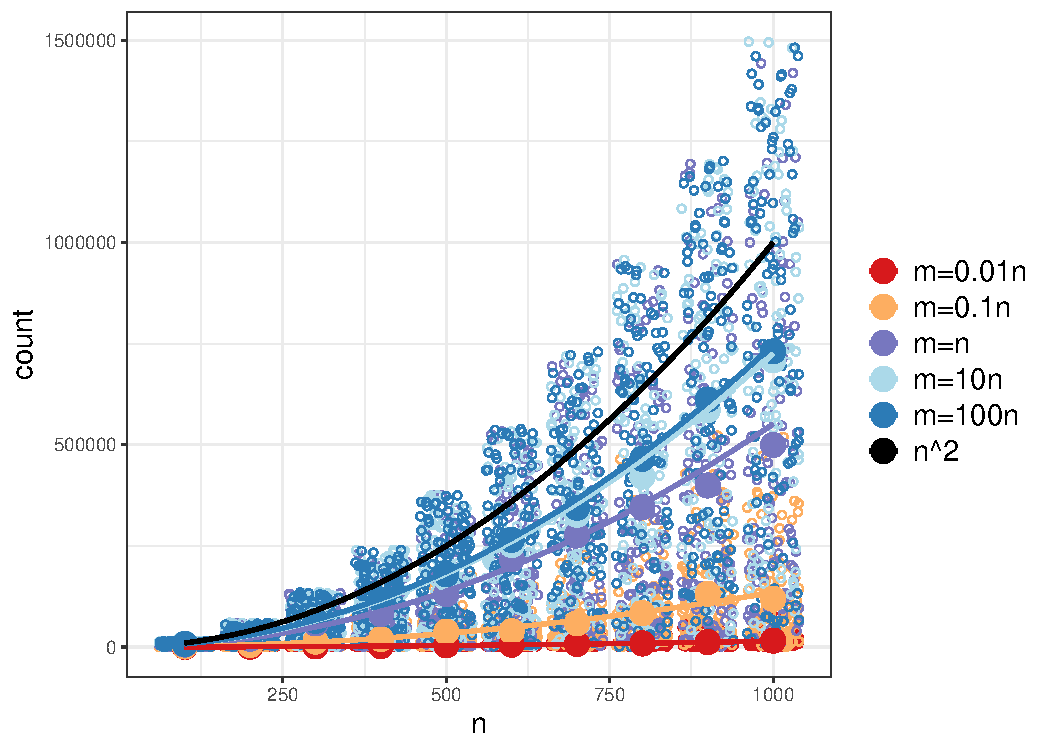
\includegraphics{report-plot1}
\caption{Operation Count vs Length of Array}
\end{figure}

\pagebreak

Figure 2. shows the average operation count scaled by its predicted efficiency class. The horizontal lines are the predicted model for each value of $m$. The lines being horizontal and the data points following them closely is a strong indicator the algorithm is of $\Theta(n^2)$.

\begin{figure}[htbp]
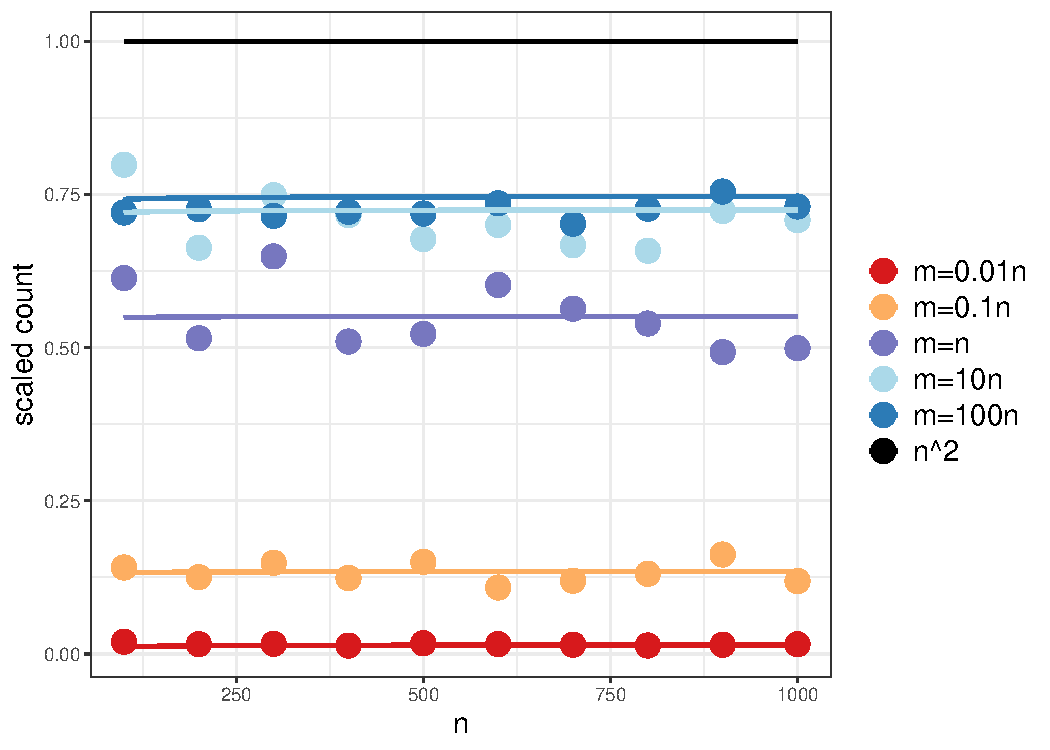
\includegraphics{report-plot2}
\caption{Scaled Average Operation Count vs Length of Array}
\end{figure}
 
\pagebreak

\subsection{Running Time}
It was conjectured in section 1.2.3 the running time would be linearly related to basic operation count. Figure 3. depicts the relationship between these two variables. The relationship appears highly correlated and linear.
\begin{align*}
time &= \beta + \alpha \cdot count + \epsilon, && \epsilon \sim Normal(0, \sigma^2) \\
time &= \hat{\alpha} \cdot count, && \hat{\alpha} = 1.1755e-06
\end{align*}
The estimate for $\alpha$ is the slope of the line of best fit for Figure 3. It will of course be dependent on system speed and is not a universal constant for the algorithm.

\begin{figure}[htbp]
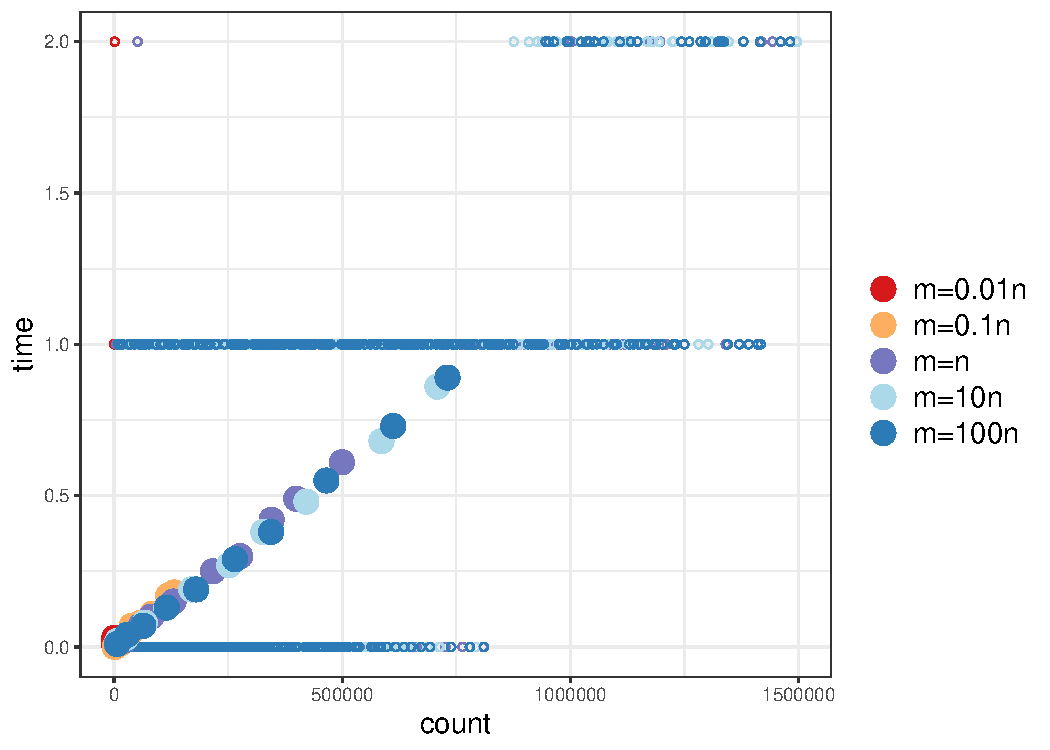
\includegraphics{report-plot3}
\caption{Operation Count vs Running Time}
\end{figure}

\pagebreak
Figure 4. shows the relationship between length of the input array and running time. The theoretical average lines are simply the model for count multiplied by $\hat{\alpha}$. The plot seems almost identical in order of growth to count, though this is hardly surprising given their correlation.

\begin{figure}[htbp]
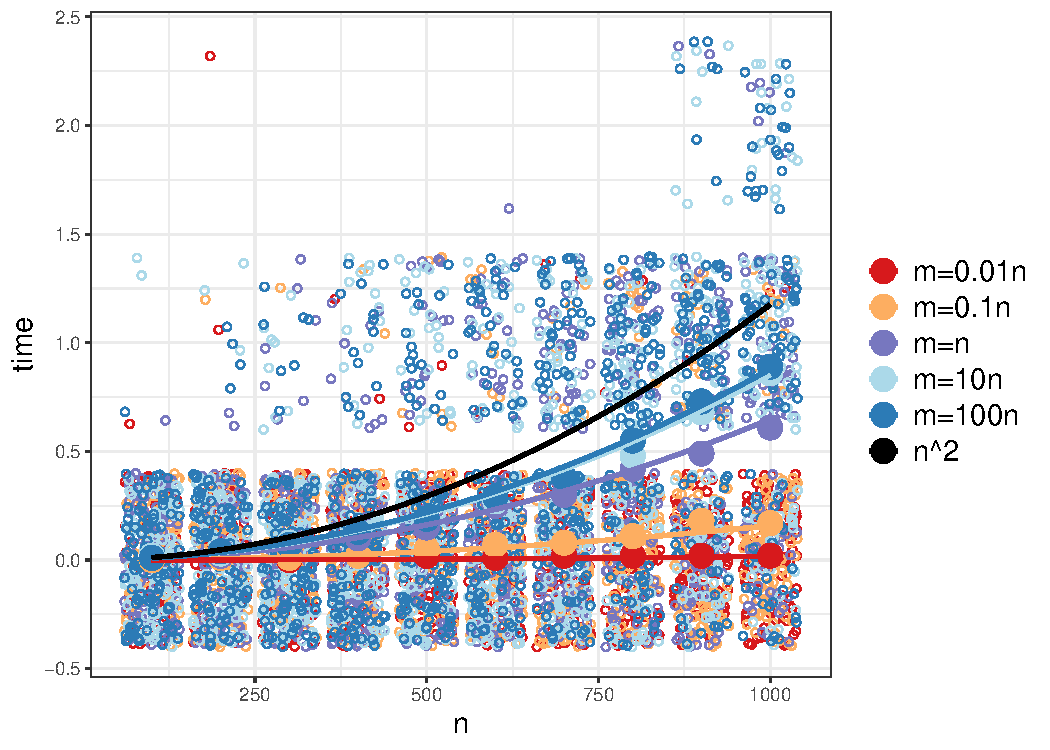
\includegraphics{report-plot4}
\caption{Running Time vs Length of Array}
\end{figure}

\pagebreak

Figure 5. was produced by the same process as in Figure 2. but for average running time. Much the same can be said regarding it, though there are some differences. While it appears the data indicates it is of $\Theta(n^2)$, the smaller values for $n$ stray from this. One cause of this could be that for smaller values of $n$ the error in time calculation is greater. It could also be random variance, though given the number of trials, it is unlikely.

\begin{figure}[htbp]
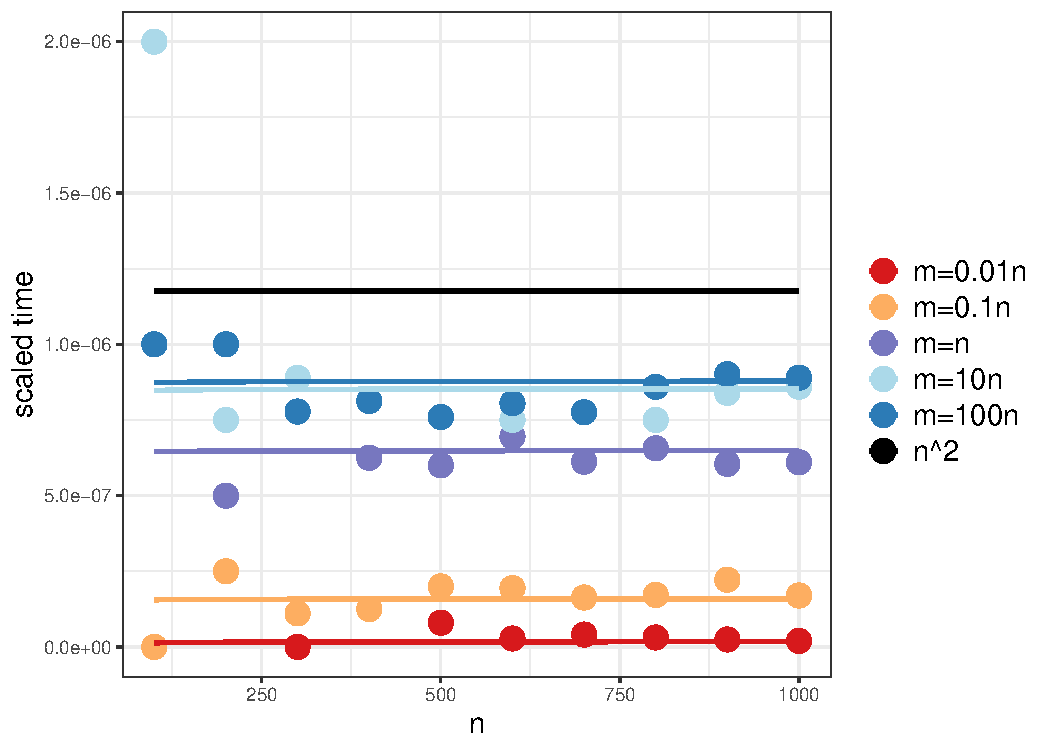
\includegraphics{report-plot5}
\caption{Scaled Average Running Time vs Length of Array}
\end{figure}



\pagebreak

\section{Conclusions}
The predicted model for the average case efficientcy fits the data well. This is especially the case for the average number of basic operations. Both observations - count and time - appear to be of $\Theta(n^2)$. The range of values sampled in the input array, $a$, also had a great effect on the speed of the algorithm. The larger values of $m$ appear to be converging to the theoretical model, $\frac{3}{4}n^2$. The smallest value of the range, $m=1$, is trivially of $\Theta(n)$. 




\end{document}
